\documentclass{llncs}
\usepackage[utf8]{inputenc}
\usepackage{amssymb}
\usepackage{stmaryrd}
\usepackage{latexsym}
\usepackage{amsmath}
\usepackage{proof}
\usepackage{stmaryrd}
\usepackage{comment}
\usepackage{pdflscape}
\usepackage[textsize=scriptsize, textwidth=2.2cm]{todonotes}
\usepackage{booktabs}
%\bibliographystyle{alpha}
% \bibliographystyle{abbrv}
\usepackage{times}

\newcommand\tsl[1]{#1}
\newcommand{\elin}[2]{\ensuremath{{\tsl{unitctx}(\ensuremath{#1}, \ensuremath{#2})}}}
\newcommand{\emp}[1]{\ensuremath{{\tsl{emp}(\ensuremath{#1})}}}
\newcommand{\eqctx}[2]{\ensuremath{{\tsl{eqctx}(\ensuremath{#1},\ensuremath{#2})}}}
\newcommand{\union}[3]{\ensuremath{{\tsl{union}(\ensuremath{#1},\ensuremath{#2},\ensuremath{ #3})}}}
\newcommand{\In}[2]{\ensuremath{\tsl{in}(\ensuremath{#1},\ensuremath{#2})}}
\newcommand{\Equ}[2]{\ensuremath{\tsl{Equ}(\ensuremath{#1},\ensuremath{#2})}}
\newcommand{\unions}[2]{\ensuremath{\tsl{Unions}(\ensuremath{#1},\ensuremath{#2})}}
\newcommand{\equal}[2]{\ensuremath{\tsl{Equal}(\ensuremath{#1},\ensuremath{#2})}}
\newcommand{\equalCtx}[2]{\ensuremath{\tsl{EqualCtx}(\ensuremath{#1},\ensuremath{#2})}}

\newcommand\Pscr{\mathcal{P}}
\newcommand{\eg}{{\em e.g.}}
\newcommand{\ie}{{\em i.e.}}
\newcommand{\etal}{\emph{et al.}}
\newcommand{\cf}{{\em cf.}}
\newcommand{\tup}[1]{\langle#1\rangle}

\newcommand{\nbang}[1]{\hbox{$!^{#1}$}}
\newcommand{\nquest}[1]{\hbox{$?^{#1}$}}

% For Quati's latex output
\newcommand{\ndots}[1]{\stackrel{\vcenter{\hbox{$\scriptstyle :$}\vskip-.35ex}}
   {\hbox {$ \scriptstyle {#1}$}}}

\title{Quati: An Automated Tool for Proving Permutation Lemmas}
\author{Vivek Nigam\inst{1} \and Giselle Reis\inst{2} \and Leonardo Lima\inst{1}}

\institute{Universidade Federal da Para\'{i}ba, Brazil
\and Technische Universit\"{a}t Wien, Austria
}

%% NOTE: 7 pages tops

%% TODO: references

\begin{document}
\maketitle

\begin{abstract}
The proof of many foundational results in structural proof theory, such as the
admissibility of the cut rule and the completeness of the focusing discipline,
rely on permutation lemmas. It is often a tedious and error prone task to prove
such lemmas as they involve many cases. This paper describes the tool Quati
which is an automated tool capable of proving a wide range of inference rule
permutations for a wide number of proof systems. Given a proof system
specification in the form of a theory in linear logic with subexponentials,
Quati outputs in \LaTeX\ the permutation transformations for which it was able
to prove correctness and also the 
possible derivations for which it was not able to do so. As illustrated in this
paper, Quati's output is very similar to proof derivation figures one would
normally find in a proof theory book. 
\end{abstract}

\vspace{-2mm}
\section{Introduction}

Permutation lemmas play an important role in proof theory. Many foundational
results about proof systems rely on the fact that some rules
permute over others. For instance, permutation lemmas are used in Gentzen-style 
cut-elimination proofs~\cite{gentzen35}, 
the completeness proof of focusing disciplines~\cite{andreoli92jlc,miller07cslb}, 
and the proof of Herbrand's theorem~\cite{herbrand30phd}.

Proving permutation lemmas, however, is often a tedious and error-prone task as there are normally many 
cases to consider. As an example, consider the case of permuting $\vee_l$ over $\rightarrow_l$ in
the intuitionistic calculus LJ. In order to show whether these two
rules permute, one needs to check \emph{every possible case} in which
$\rightarrow_l$ occurs above $\vee_l$ in a derivation. When using a
multiplicative calculus, there are four possibilities for such derivation, two
allow a permutation of the rules while the other two do not.
% \footnote{In an additive calculus there are three possibilities, only one of them allow a
% permutation.} 
Here's one of each:
%% -> l / v l
\vspace{-4mm}

{\scriptsize
\[
\infer[\vee_l]{\Gamma, \Gamma', \Gamma'', A \rightarrow B , P \vee Q \vdash F}{
  \deduce{\Gamma, P \vdash F}{\varphi_1\vspace{0.2cm}}
  &
  \infer[\rightarrow_l]{\Gamma', \Gamma'', A \rightarrow B , Q \vdash F}{
    \deduce{\Gamma' \vdash A}{\varphi_2\vspace{0.2cm}}
    &
    \deduce{\Gamma'', Q, B \vdash F}{\varphi_3\vspace{0.2cm}}
  }
}
\quad\rightsquigarrow\quad
\infer[\rightarrow_l]{\Gamma, \Gamma', \Gamma'', P \vee Q, A \rightarrow B
\vdash F}{
  \deduce{\Gamma' \vdash A}{\varphi_2\vspace{0.2cm}}
  &
  \infer[\vee_l]{\Gamma, \Gamma'', P \vee Q, B \vdash F}{
    \deduce{\Gamma, P \vdash F}{\varphi_1\vspace{0.2cm}}
    &
    \deduce{\Gamma'', B, Q \vdash F}{\varphi_3\vspace{0.2cm}}
  }
}
\]
}
%% -> l / v l
% \vspace{-2mm}
{\scriptsize
\[
\infer[\vee_l]{\Gamma, \Gamma', \Gamma'', A \rightarrow B , P \vee Q \vdash F}{
  \deduce{\Gamma, P \vdash F}{\varphi_1\vspace{0.2cm}}
  &
  \infer[\rightarrow_l]{\Gamma', \Gamma'', A \rightarrow B , Q \vdash F}{
    \deduce{\Gamma', Q \vdash A}{\varphi_2\vspace{0.2cm}}
    &
    \deduce{\Gamma'', B \vdash F}{\varphi_3\vspace{0.2cm}}
  }
}
\quad\rightsquigarrow\quad
?
\]
}%
The combinatorial nature of the proof of permutation lemmas can be observed in
this example. While there are ``only'' four cases to consider for this pair of rules, for
proving the completeness of the focusing discipline, one needs to study which
permutations are allowed and therefore all pairs of rules need to be
considered~\cite{miller07cslb}.
Moreover, the fact that the cases are rarely documented makes it hard for others to check the
correctness of the transformations. For instance, the cut-elimination result for
bi-intuitionistic logic given by Rauszer \cite{rauszer74studia}
was later found to be incorrect \cite{crolard01tcs} exactly because one of the
permutation lemmas was not true. Therefore, an automated tool to check for these lemmas
would be of great help. This paper introduces such a tool called Quati.

While here we will restrict ourselves to simply illustrate Quati's
functionalities and implementation design, we observe that its underlying theory
is described in the papers~\cite{nigam.jlc,nigam13iclp,nigam14ebl}. We briefly
review this body of work.  
 
In~\cite{nigam13iclp}, we show how to reduce the problem of proving permutation
lemmas to solving an answer-set program~\cite{gelfond90iclp}. That is given a proof
system, $\Pscr$, satisfying some properties, we reduce the problem 
of checking whether a rule $r_1$ in $\Pscr$ always permutes over $r_2$ in
$\Pscr$ to solving an answer-set program. Each solution of this program
corresponds to one possible permutation case. This result sets the foundations 
for Quati.

However, the exact language in which proof systems are specified was not dealt
in~\cite{nigam13iclp}. It was subject of the paper~\cite{nigam.jlc} which
shows that a great number of proof systems for different logics (\eg, linear,
intuitionistic, classical, modal logics) can be specified as theories in linear
logic with subexponentials (SELL)~\cite{nigam09ppdp}. These specifications are shown to
have a strong adequacy, namely, \emph{on the level of
derivations}~\cite{nigam10jar}, meaning that there is a one to one
correspondence of derivations in the specified logic (object logic) to derivations in linear
logic with subexponentials. Moreover, \cite{nigam.jlc} also shows how to check whether 
proof systems specified in SELL admit cut-elimination. This lead to the tool 
TATU\footnote{\url{https://www.logic.at/staff/giselle/tatu/}.} Therefore, SELL is
a suitable framework for specifying proof systems. 

Finally, in the workshop paper~\cite{nigam14ebl}, we show how to integrate the material
in \cite{nigam13iclp} and \cite{nigam.jlc}. In particular, we show how to reduce,
to solving an answer-set program, the problem of checking whether a rule permutes
over another when given a proof system specified in SELL. 
Moreover, we also discuss in \cite{nigam14ebl} how to extract
proof derivation figures similar to those shown in a standard proof theory
book~\cite{troelstra96bpt} from the solutions of the generated answer-set programs. 

Quati is the result of this series of papers. This paper is organized as follows: Section~\ref{sec:quati} describes
Quati's syntax and its features, while Section~\ref{sec:impl} describes its implementation.
In Section~\ref{sec:conc} we end by pointing out future work.

\vspace{-4mm}

\section{Quati at Work}
\label{sec:quati}

Throughout this section, we will use the specification for the
intuitionistic logic's multi-conclusion calculus MLJ \cite{maehara54nmj} as our running 
example. First we specify Quati's syntax and then its features. In the Appendix
you can find step-by-step use of the Quati system for this example as well as the proof system MLJ. 

\vspace{-2mm}

\subsection{Syntax}

% TODO: fix this table once everything is there.
\begin{figure}[t]
{\small
\[
\begin{array}{lcl}
Side ::= \texttt{lft} \;\;|\;\; \texttt{rght} \quad 
CtxType ::=  \texttt{many} \;\;|\;\; \texttt{single} \quad
SubType ::=  \texttt{unb} \;\;|\;\; \texttt{lin} \\[2pt]
SubSig ::= SubDecl \;\; SubSpec \;\; SubRel \\[2pt]
SubDecl ::= \texttt{subexp} \tup{String} \tup{SubType}.\\[2pt]
SubSpec ::= \texttt{subexpctx} \tup{String} \tup{CtxType} \tup{Side}.\\[2pt]
SubRel ::= \texttt{subexprel} \tup{String} \texttt{<} \tup{String}. \\[2pt]
Bipoles ::= (\texttt{not} \tup{Atoms}) \texttt{*} \tup{BodyPos}. \\[2pt]
BodyPos ::=\texttt{one} \;\;|\;\; BodyNeg \;\;|\;\; \texttt{[}\tup{String}\texttt{]bang} BodyNeg \;\;|\;\;\\ 
        \qquad\qquad BodyPos \texttt{*} BodyPos \;\;|\;\; BodyPos \texttt{+} BodyPos \\[2pt]
BodyNeg ::= \texttt{top} \;\;|\;\; \texttt{bot} \;\;|\;\; \tup{MarkAtoms} \;\;|\;\; \tup{BodyNeg}|\tup{BodyNeg} \;\;|\;\; \\
        \qquad \qquad \tup{BodyNeg} \texttt{\&} \tup{BodyNeg}\\[2pt]
Atoms ::=\tup{Side} \tup{Form} \qquad MarkAtoms ::=  \texttt{[}\tup{String}\texttt{]?} \tup{Atoms} \\
\end{array}
\]
% \begin{align*}
% SubSig &::= SubDecl \;\; SubSpec \;\; SubRel \\
% SubDecl &::= \texttt{subexp} \tup{String} \tup{SubType}.\\
% SubSpec &::= \texttt{subexpctx} \tup{String} \tup{CtxType} \tup{Side}.\\
% SubRel &::= \texttt{subexprel} \tup{String} \texttt{<} \tup{String}. \\
% Side &::= \texttt{lft} \;\;|\;\; \texttt{rght} \\
% CtxType &::=  \texttt{many} \;\;|\;\; \texttt{single} \\
% SubType &::=  \texttt{unb} \;\;|\;\; \texttt{lin} \\
% Bipoles &::= (\texttt{not} \tup{Atoms}) \texttt{*} \tup{BodyPos}. \\
% Atoms &::= \tup{Side} \tup{Form} \\
% BodyPos &::= \texttt{one} \;\;|\;\; BodyNeg \;\;|\;\; \texttt{[}\tup{String}\texttt{]bang} BodyNeg \;\;|\;\;\\ 
%         & BodyPos \texttt{*} BodyPos \;\;|\;\; BodyPos \texttt{+} BodyPos \\
% BodyNeg &::= \texttt{top} \;\;|\;\; \texttt{bot} \;\;|\;\; \tup{MarkAtoms} \;\;|\;\; \tup{BodyNeg}|\tup{BodyNeg} \;\;|\;\; \\
%         & \tup{BodyNeg} \texttt{\&} \tup{BodyNeg}\\
% MarkAtoms &::= \texttt{[}\tup{String}\texttt{]?} \tup{Atoms} 
% \end{align*}
}
\vspace{-4mm}
% \textbf{VN: We need to add more constructs}
\caption{Here $Form$ is a term of type \texttt{form}.} 
\label{fig:syntax}
\begin{center}
\begin{tabular}{c@{\quad}c@{\quad}c@{\quad}c@{\quad}c@{\quad}c@{\quad}c@{\quad}c@{\quad}c@{\quad}c}
\toprule
\texttt{*} : $\otimes$ & \texttt{+} : $\oplus$ & \texttt{\&} : $\&$ & \texttt{|} : $\bindnasrepma$ & \texttt{[i]bang} : $!^i$ &
\texttt{one} : $1$ &  \texttt{top} : $\top$ & \texttt{bot} : $\bot$ & \texttt{[i]?} : $?^i$ \\
\bottomrule
\end{tabular}
\end{center}
\vspace{-4mm}
\caption{Syntax for the linear logic connectives.}
\label{fig:syntax_ll}
\vspace{-4mm}
\end{figure}

Quati's underlying logic, linear logic with subexponentials
(SELL)~\cite{nigam09ppdp}, is a powerful framework for the specification of proof systems. 
Subexponentials, written $\nbang{\ell}$, $\nquest{\ell}$, arise from the
observation that the linear logic exponentials are not canonical (see
\cite{nigam.jlc} for an extensive discussion). It is known that these operators
greatly increase
the expressiveness of the system when compared to linear logic. For instance,
subexponentials can be used to represent contexts of proof
systems~\cite{nigam.jlc}, to mark the epistemic state of
agents~\cite{nigam12lics}, or to specify locations in sequential
computations~\cite{nigam09ppdp}. 
The main feature of subexponentials is that they can be organized in a pre-order, $\preceq$, which specifies
the provability relation among them. 
In \cite{nigam.jlc}, we have shown that a wide number of proof systems for linear, classic, intuitionistic and 
modal logics can be specified in SELL with a strong level of adequacy. 

Another important reason for using SELL as specification language is that one can also use 
other available tools, such as the tool TATU which is capable to check whether a proof system 
specified in SELL admits cut-elimination.

A Quati program is a SELL theory with some more annotations. Its syntax is given
in Figure~\ref{fig:syntax} and explained in detail  
by using as running example the inference rules of the multiconclusion sequent
calculus for intuitionistic logic~\cite{maehara54nmj}, or MLJ.

A Quati program consists of two files: (1) a \emph{type signature} file, with
suffix \texttt{.sig} and (2) a specification file with suffix \texttt{.pl} consisting of two parts: (a) a
\emph{subexponential signature} and (b) the rules' specifications or
\emph{bipoles}.

\vspace{-2mm}

\paragraph{Type signature}
%
The \emph{type signature} file contains type and kind declarations of the object
logic's elements. The kind \texttt{form} is built-in and
represent the type of formulas of the object logic. In general, only
the types of the connectives need to be declared in this file. Here is an
example:
\vspace{-1mm}

{\small
\begin{verbatim}
%%%%%%%%%%%%%%%%%%% Signature %%%%%%%%%%%%%%%%%%%%
type imp form -> form -> form.
\end{verbatim}
}

\paragraph{Subexponential signature}
%
The following subexponential signature is used for specifying the proof system MLJ:
\vspace{-1mm}

{\small
\begin{verbatim}
%%%%%%%%%%%%%%% Subexponential Signature %%%%%%%%%%%%%%%%%
subexp l unb.                       subexp r unb.            
subexpctx l many lft.               subexpctx r many rght.
subexprel l > r
\end{verbatim}
}

Intuitively, one subexponential corresponds to one context of the object logic sequent.\footnote{There are 
some specifications where a subexponential is used to capture the structural properties of the proof 
system and therefore does not necessarily correspond to a context in the object logic. See \cite{nigam.jlc}
for more on this.}
For MLJ, as it has only two
contexts, one to the left and another to the right side of the sequent, we use two subexponentials
\texttt{l} and \texttt{r}. Moreover, as both contexts (to the left and right) behave classically in MLJ, 
we specify \texttt{l} and \texttt{r} to be unbounded, denoted by \texttt{unb}. In contrast, 
the specification of LJ would specify the subexponential \texttt{r} to be linear, as the right side of LJ's 
sequents behaves linearly.

The commands \texttt{subexpctx l many lft.} and  \texttt{subexpctx r many rght.} are not formally needed for specifying proof systems, 
but as discussed 
in \cite{nigam14ebl}, they are needed in order to improve the visualization of the proof rules. 
In particular, the former specifies that the context corresponding to the subexponential \texttt{l} contains 
only formulas of the left side of the sequent, denoted by \texttt{lft}, and may contain many formulas, denoted 
by \texttt{many}. In contrast, as the context to the right side of LJ sequents has only one formula, the 
subexponential \texttt{r} for that system would be annotated with \texttt{single}.

The pre-order among the subexponentials is specified on the last line using the
keyword \texttt{subexprel}.

\vspace{-2mm}

\paragraph{Bipoles}
%
The second part of the \texttt{.pl} file is composed by $bipoles$. The concrete syntax for SELL connectives
is depicted in Figure~\ref{fig:syntax_ll}. The class of $bipole$ formulas often
appear in proof theory literature due to its good focusing
behaviour~\cite{andreoli92jlc}. The following bipoles specify, 
respectively, the left and right implication introduction rules~\cite{nigam.jlc}. The capital 
letters are assumed to be existentially quantified.
\vspace{-1mm}

% TODO: explain the division into rule types??? No. No space.
{\small
\begin{verbatim}
%%%%%%%%%%%%%%%%%%%%%%%%%% Bipoles %%%%%%%%%%%%%%%%%%%%%%%%%%%
% Implication
(not (lft (imp A B))) * (([r]? (rght A)) * ([l]? (lft B))).
(not (rght (imp A B))) * [l]bang (([l]? (lft A)) | ([r]? (rght B))).
\end{verbatim}
}

The head of these bipoles, the formulas \texttt{(not (lft (imp A B)))} and
\texttt{(not (rght (imp A B)))}, specify that an implication formula to, respectively, 
the left and right-hand-side is introduced. The body specifies the premises of these
rules. For instance, the first bipole specifies that its corresponding inference rules
has two premises because of the branching caused by the  
tensor \texttt{*} appearing in the body of its rule, while
the second has only one premise as no branching is required. 
The interesting bit is the bang \texttt{[l]bang} in second bipole specifying that the 
context of the subexponential \texttt{r} should be weakened as \texttt{l > r}.
In fact, by using advanced proof theoretic machinery, namely Focusing~\cite{andreoli92jlc}, 
we can make this intuition precise in the sense. We refer to~\cite{nigam.jlc} for more details
on encodings.

% \vspace{-3mm}

\subsection{Features}

Quati has two main features: (1) It can construct the corresponding inference rule(s) associated
to a SELL formula; and (2) it can prove permutation lemmas. We illustrate these features with 
the specification of MLJ implication introduction rules shown above.

\vspace{-2mm}

\paragraph{Rule Construction} Proving the adequacy theorems for a given SELL specification is also 
error-prone. As detailed~\cite{nigam.jlc}, to prove (strong) adequacy we need to show that all 
the possible focused derivations that introduce a formula in the specification corresponds to 
an inference rule of the proof system being specified. Quati automates the proof of such 
adequacy theorems by constructing from a bipole the corresponding inference rule formulas. 
To do so, Quati uses the machinery described in \cite{nigam13iclp,nigam14ebl} reducing
this problem to the problem of solving answer-set programs. 

For the MLJ specification given above, one can use the command \texttt{\#rule} in the command 
line and select a SELL bipole in the loaded specification. Then Quati generates all possible 
inference rules that correspond to that bipole written in \LaTeX. If we select the bipole used to specify 
MLJ's implication right rule, Quati outputs the \LaTeX\ code for the following figure:
\vspace{-3mm}

{\small
\[
\cfrac{ \ndots{l} \Gamma_{l}^{0}, a \vdash  \ndots{r} b}
{ \ndots{l} \Gamma_{l}^{0} \vdash  \ndots{r} \Delta_{r}^{0}, imp (a) (b) } \;\; imp_{R}
\]
}

Notice that this rule looks very similar to MLJ's implication right introduction rule shown in any proof theory 
textbook. The context $\Delta_{r}^{0}$ is erased in the premise. The $\ndots{l}$ and $\ndots{r}$ are used to 
delimit the contexts for the subexponentials \texttt{l} and \texttt{r}, respectively. Quati uses the subexponential 
specification to infer that the context for \texttt{l} (resp. for \texttt{r}) should only to the left-hand-side (resp. 
right-hand-side) of the sequent.

Under the hood, Quati is constructing the focused derivation~\cite{andreoli92jlc} that introduces such 
a SELL bipole as described in \cite{nigam.jlc}. This can be observed by using the command 
\texttt{bipole}. For the same SELL bipole used above, Quati returns
the \LaTeX\ code for the following figure, corresponding to the focused derivation of the SELL bipole:
\vspace{-4mm}


{\scriptsize\[\cfrac{\cfrac{\cfrac{}
{\Gamma_{ gamma}^{4} ; \Gamma_{r}^{4} ; \Gamma_{l}^{3} ; \Gamma_{ infty}^{1} ;  \Downarrow \neg rght (imp (a) (b) )  } \quad \cfrac{\cfrac{\cfrac{\cfrac{\Gamma_{ gamma}^{5} ; \Gamma_{r}^{7} ; \Gamma_{l}^{5} ; \Gamma_{ infty}^{1} ;  \Uparrow }
{\Gamma_{ gamma}^{5} ; \Gamma_{r}^{5} ; \Gamma_{l}^{5} ; \Gamma_{ infty}^{1} ;  \Uparrow  ?^{r} rght (b)  }}
{\Gamma_{ gamma}^{5} ; \Gamma_{r}^{5} ; \Gamma_{l}^{3} ; \Gamma_{ infty}^{1} ;  \Uparrow  ?^{l} lft (a)  ::  ?^{r} rght (b) }}
{\Gamma_{ gamma}^{5} ; \Gamma_{r}^{5} ; \Gamma_{l}^{3} ; \Gamma_{ infty}^{1} ;  \Uparrow  ?^{l} lft (a)  \bindnasrepma  ?^{r} rght (b)  }}
{\Gamma_{ gamma}^{5} ; \Gamma_{r}^{4} ; \Gamma_{l}^{3} ; \Gamma_{ infty}^{1} ;  \Downarrow  !^{l}  ?^{l} lft (a)  \bindnasrepma  ?^{r} rght (b)  }}
{\Gamma_{ gamma}^{3} ; \Gamma_{r}^{4} ; \Gamma_{l}^{3} ; \Gamma_{ infty}^{1} ;  \Downarrow \neg rght (imp (a) (b) )  \otimes  !^{l}  ?^{l} lft (a)  \bindnasrepma  ?^{r} rght (b) }}
{\Gamma_{ gamma}^{3} ; \Gamma_{r}^{4} ; \Gamma_{l}^{3} ; \Gamma_{ infty}^{1} ; \Uparrow }\]}


\vspace{-2mm}

\paragraph{Rule Permutation}
As described in the Introduction, Quati can be used to prove permutation lemmas. The command \texttt{\#permute} in the command 
line checks whether the permutation of two selected rules is always allowed or not. Quati outputs, again in \LaTeX, the cases for
which it was able to find the permutation and the cases for which it was not able to find a permutation. For example, when Quati 
checks whether MLJ's implication left introduction rule permutes over MLJ's implication right introduction, Quati correctly finds two possible
permutation cases and it cannot find one of the cases for which is indeed not possible. We show one of the cases (reformated to fit the page margins):
\vspace{-3mm}

{\scriptsize
\[
\begin{array}{ll}
\cfrac{\cfrac{ \ndots{l} \Gamma_{l}^{0}, imp (a) (b) , c \vdash  \ndots{r} d}
{ \ndots{l} \Gamma_{l}^{0}, imp (a) (b)  \vdash  \ndots{r} \Delta_{r}^{0}, imp (c) (d) , a} \;\; imp_{R}
\quad
 \ndots{l} \Gamma_{l}^{0}, imp (a) (b) , b \vdash  \ndots{r} \Delta_{r}^{0}, imp (c) (d) }
{ \ndots{l} \Gamma_{l}^{0}, imp (a) (b)  \vdash  \ndots{r} \Delta_{r}^{0}, imp (c) (d) } \;\; imp_{L}\\\\
\qquad \qquad \qquad \qquad \qquad \qquad \qquad \quad\rightsquigarrow\quad
\cfrac{\cfrac{ \ndots{l} \Gamma_{l}^{7}, imp (a) (b) , c \vdash  \ndots{r} a, d
\quad
 \ndots{l} \Gamma_{l}^{7}, imp (a) (b) , c, b \vdash  \ndots{r} d}
{ \ndots{l} \Gamma_{l}^{7}, imp (a) (b) , c \vdash  \ndots{r} d} \;\; imp_{L}}
{ \ndots{l} \Gamma_{l}^{7}, imp (a) (b)  \vdash  \ndots{r} \Delta_{r}^{9}, imp (c) (d) } \;\; imp_{R}
\end{array}
\]
}

Once again, this proof figure is very similar to the proof figure that one would find in a standard proof theory textbook.
Notice that it uses the fact that the contexts are unbounded to infer the permutation above (see \cite{nigam13iclp} for 
more discussion on how this).

\section{Implementation Details}
\label{sec:impl}

Quati is implemented in OCaml\footnote{\url{http://ocaml.org/}} and makes use of
DLV\footnote{\url{http://www.dlvsystem.com/dlv/}} externally to compute minimal models for the
answer-set programs generated. It is part of a bigger project, called
\texttt{sellf}\footnote{\url{https://code.google.com/p/sellf/}} which also includes the
machinery for TATU mentioned above. 

The basic data structure is linear logic formulas,
defined in the \texttt{Term} module. Figure \ref{fig:modules} is an overview
of the modules in \texttt{sellf} used by Quati to check for permutations.

\begin{figure}
TODO: module's figure
\end{figure}

\textbf{Add a paragraph on the results, such as time to compute, which systems, etc.}

\textbf{TODO:} wait for the picture to explain in more detail the modules and how they
interact.

\section{Conclusions and Future Work}
\label{sec:conc}
This paper introduced Quati an automated tool for proving permutation lemmas. Besides briefly 
comenting on its implementation, we illustrated its syntax, usage and features. Besides MLJ, in the release
one can find a number of implemented systems, such as systems for linear logic, intuitionistic logic, s4, 
and others. 

There is a number of directions that we are currently investigating. One direction is to come up with 
more graphical ways of writing proof systems and how to translate such representations into SELL specifications. 
Since the proof of the completeness theorem of focusing strategies heavily rely on permutation lemmas, we are 
currently investigating ways to derive such theorems in an automated fashion. Finally, we are investigating
ways to construct machine-readable proof objects for permutation lemmas.

\bibliographystyle{abbrv}
\bibliography{../master}


% \section{A Multiconclusion Sequent Calculus for Intuitionistic Logic}



\newpage
\appendix

\begin{figure}
\[
\begin{array} {r@{\quad}l}
\infer[{\supset_L}]{\Gamma, A\supset B \longrightarrow \Delta}{\Gamma,
A\supset B \longrightarrow A, \Delta \quad \Gamma,A\supset B, B \longrightarrow
\Delta }
&
\infer[{\supset_R}]{\Gamma \longrightarrow A \supset B, \Delta}{\Gamma, A
\longrightarrow B}
\\[5pt]
\infer[{\land_L}]{\Gamma, A \land B \longrightarrow \Delta}{\Gamma, A \land
B, A,B \longrightarrow \Delta }
&
\infer[{\land_R}]{\Gamma \longrightarrow A \land B, \Delta}{\Gamma \longrightarrow
A \land B, A, \Delta \quad \Gamma \longrightarrow A \land B,B, \Delta}
\\
[5pt]
\infer[{\lor_L}]{\Gamma, A \lor B \longrightarrow  \Delta}{\Gamma, A \lor B,
A, \longrightarrow \Delta \quad \Gamma, A \lor B,B \longrightarrow  \Delta}
&
\infer[{\lor_R}]{\Gamma \longrightarrow A \lor B, \Delta}{\Gamma \longrightarrow A
\lor B, A,B, \Delta }
\\
[5pt]
\infer[{\forall_L}]{\Gamma, \forall x\,A \longrightarrow \Delta}{\Gamma,
\forall x\,A, A\{t/x\} \longrightarrow \Delta} 
&
\infer[{\forall_R}]{\Gamma \longrightarrow \Delta, \forall x\,A}{\Gamma
\longrightarrow A\{c/x\}}
\\
[5pt]
\infer[{\exists_L}]{\Gamma, \exists x\, A \longrightarrow
\Delta}{\Gamma, \exists x\, A , A\{c/ x\} \longrightarrow \Delta} 
&
\infer[{\exists_R}]{\Gamma \longrightarrow \Delta, \exists x\, A}
{\Gamma \longrightarrow \Delta, \exists x\, A, A \{t/x\}}
\end{array}
\]
%\end{small}
% \vspace{-4mm}
%\begin{small}
\[
\begin{array}{c@{\qquad}c@{\qquad}c}
 \infer[{\textrm{Init}}]{\Gamma,A \longrightarrow A, \Delta}{} 
&
\infer[{\textrm{Cut}}]{\Gamma \longrightarrow \Delta}{\Gamma
\longrightarrow B,\Delta \quad \Gamma, B \longrightarrow \Delta}
&
\infer[{\bot_L}]{\Gamma,\bot \longrightarrow \Delta}{} 
\end{array}
\]
%\end{small}
% \vspace{-4mm}
\caption{The multi-conclusion intuitionistic sequent calculus, MLJ,
with additive rules.}\label{Fig:mLJ}
% \vspace{-4mm}
\end{figure}


\section{A sample Quati session}
% TODO: add installation instructions and system requirements, explain where the
% examples are? Or just refer the reader to the download and add these things to
% a readme file...

% TODO: change executable file name for quati in the release
% load a file
Once the system in build,\footnote{Notice that one needs Ocaml and DLV systems installed to make
Quati work.} it can be called by simply typing the command:
\texttt{./quati}. This will start an interactive command line where the user can
call the functions we will demonstrate now. If one wants to see a list of all
the functionalities available, just type \texttt{\#help}. We start by loading a
file. Throughout this example session, we will use the specification for the
intuitionistic logic's multi-conclusion calculus MLJ \cite{maehara54nmj}.
%
\vspace{-1mm}

{\small
\begin{verbatim}
:> #load ../examples/proofsystems/mlj
\end{verbatim}
}

% construct OL rule (for one and for all)
After a file is loaded, the state of the command line will change from
\texttt{:>} to \texttt{?>}. This indicates that the user can use the commands
operating on a specification. The first command we show is \texttt{\#rule} or
\texttt{\#rules}. It allows the user to see the rules specified in the file
loaded as regular sequent calculus rules. In both cases, the system prints the
rule or rules in a \LaTeX\ file whose name is chosen by the user. By using the
command \texttt{\#rule}, the user is presented with the list of bipoles of the
loaded specification and asked to choose one. The object logic rule for this
bipole is then printed to a file. By using the command \texttt{\#rules}, the
object logic rules of all bipoles are printed to the output file. In the example
below, we asked Quati to print the rule for $\rightarrow_r$ of the MLJ system.
\vspace{-1mm}

{\small
\begin{verbatim}
?> #rule
These are the formulas available: 
0. (sigma \B (sigma \A (not ( lft ( imp A B  )  ))  * 
   ( [r]? ( rght A  ) ) * ( [l]? ( lft B  ) )))
1. (sigma \B (sigma \A (not ( rght ( imp A B  )  ))  * 
   ( [l]bang ( [l]? ( lft A  ) ) | ( [r]? ( rght B  ) ) )))
The object logic rule of the chosen formula will be generated 
and printed to a LaTeX file.
Please choose a formula by its number: 1
Please choose a name for the file: imp_r_mlj
\end{verbatim}
}

This is the output (after compiling with \LaTeX):
%
{\small
\[
\cfrac{ \ndots{l} \Gamma_{l}^{0}, a \vdash  \ndots{r} b}
{ \ndots{l} \Gamma_{l}^{0} \vdash  \ndots{r} \Delta_{r}^{0}, imp (a) (b) } \;\; imp_{R}
\]
}

Note that the rule has the expected behavior of weakening the formulas of the
context on the right, and it is very similar to the way it is presented in text
books.

% construct bipole (for one and for all)
The user has also the option of seeing the actual bipole derivations in linear
logic with subexponentials which correspond to a rule specification. The
commands \texttt{\#bipole} and \texttt{\#bipoles} are used for that. They work
analogously to the previous commands. The example below shows how to use
\texttt{\#bipole} to print the bipole corresponding to the $\rightarrow_r$ rule
of MLJ.
\vspace{-1mm}

{\small
\begin{verbatim}
?> #bipole 
These are the formulas available: 
0. (sigma \B (sigma \A (not ( lft ( imp A B  )  ))  * 
   ( [r]? ( rght A  ) ) * ( [l]? ( lft B  ) )))
1. (sigma \B (sigma \A (not ( rght ( imp A B  )  ))  * 
   ( [l]bang ( [l]? ( lft A  ) ) | ( [r]? ( rght B  ) ) )))
The bipoles for the chosen formula will be generated and printed to a LaTeX file.
Please choose a formula by its number: 1
Please choose a name for the file: bipole_imp_r_mlj
\end{verbatim}
}

The output of this command generates the following proof tree:
%
{\scriptsize\[\cfrac{\cfrac{\cfrac{}
{\Gamma_{ gamma}^{4} ; \Gamma_{r}^{4} ; \Gamma_{l}^{3} ; \Gamma_{ infty}^{1} ;  \Downarrow \neg rght (imp (a) (b) )  :: }\cfrac{\cfrac{\cfrac{\cfrac{\Gamma_{ gamma}^{5} ; \Gamma_{r}^{7} ; \Gamma_{l}^{5} ; \Gamma_{ infty}^{1} ;  \Uparrow }
{\Gamma_{ gamma}^{5} ; \Gamma_{r}^{5} ; \Gamma_{l}^{5} ; \Gamma_{ infty}^{1} ;  \Uparrow  ?^{r} rght (b)  :: }}
{\Gamma_{ gamma}^{5} ; \Gamma_{r}^{5} ; \Gamma_{l}^{3} ; \Gamma_{ infty}^{1} ;  \Uparrow  ?^{l} lft (a)  ::  ?^{r} rght (b)  :: }}
{\Gamma_{ gamma}^{5} ; \Gamma_{r}^{5} ; \Gamma_{l}^{3} ; \Gamma_{ infty}^{1} ;  \Uparrow  ?^{l} lft (a)  \bindnasrepma  ?^{r} rght (b)  :: }}
{\Gamma_{ gamma}^{5} ; \Gamma_{r}^{4} ; \Gamma_{l}^{3} ; \Gamma_{ infty}^{1} ;  \Downarrow  !^{l}  ?^{l} lft (a)  \bindnasrepma  ?^{r} rght (b)  :: }}
{\Gamma_{ gamma}^{3} ; \Gamma_{r}^{4} ; \Gamma_{l}^{3} ; \Gamma_{ infty}^{1} ;  \Downarrow \neg rght (imp (a) (b) )  \otimes  !^{l}  ?^{l} lft (a)  \bindnasrepma  ?^{r} rght (b)  :: }}
{\Gamma_{ gamma}^{3} ; \Gamma_{r}^{4} ; \Gamma_{l}^{3} ; \Gamma_{ infty}^{1} ; \Uparrow }\]}

By using the rewrite system introduced in \cite{nigam13iclp}, Quati is able to
translate this bipole into the previous inference rule.

% permute (for two and for all)
Now let's show how to actually check if two of these rules permute. The commands
to do that are \texttt{\#permute} and \texttt{\#permute\_all}. As one can
imagine, the former will check the permutation of two rules that are chosen by
the user, while the latter will check the permutation of every pair of rules in
the specification file. The output of this command is also a \LaTeX\ file. It
contains the cases in which a permutation was found as well as the cases in
which a permutation was not found. Let's try a permutation in our example:
\vspace{-1mm}

{\small
\begin{verbatim}
?> #permute
These are the formulas available: 
0. (sigma \B (sigma \A (not ( lft ( imp A B  )  ))  * 
   ( [r]? ( rght A  ) ) * ( [l]? ( lft B  ) )))
1. (sigma \B (sigma \A (not ( rght ( imp A B  )  ))  * 
   ( [l]bang ( [l]? ( lft A  ) ) | ( [r]? ( rght B  ) ) )))
Checking the permutation of one formula F1 over another F2 
(i.e., can a derivation where F1 is below F2 be transformed into a derivation 
where F2 is below F1) 
Please type the number of F1: 0
Please type the number of F2: 1
Please type a file name for the results: imp_l_imp_r
\end{verbatim}
}

The output file of this command indicates the these rules might not permute.
Quati identifies permutation for two cases but fails to find for the third one.
Its output for the permutation case is depicted in Section~\ref{sec:permutation} 
after compiling in \LaTeX:

\begin{landscape}
%\documentclass[a4paper]{article}
%\usepackage[utf8]{inputenc}
%\usepackage{amsmath}
%\usepackage{amssymb}
%\usepackage{stmaryrd}
%\usepackage{proof}

%\usepackage[paperwidth=25cm, paperheight=13cm, margin=1cm]{geometry}
%\usepackage[landscape, margin=1cm]{geometry}

%\newcommand{\ndots}[1]{\stackrel{\vcenter{\hbox{$\scriptstyle :$}\vskip-.35ex}}
%   {\hbox {$ \scriptstyle {#1}$}}}

%\begin{document}
\pagestyle{empty}
\section{Permutation of $imp_{lft}$ and $imp_{rght}$}
\label{sec:permutation}
The rules might not permute. These are the configurations for which a permutation was found:
{\scriptsize
\[
\cfrac{\cfrac{ \ndots{l} \Gamma_{l}^{0}, imp (a) (b) , c \vdash  \ndots{r} d}
{ \ndots{l} \Gamma_{l}^{0}, imp (a) (b)  \vdash  \ndots{r} \Delta_{r}^{0}, imp (c) (d) , a} \;\; imp_{R}
\quad
 \ndots{l} \Gamma_{l}^{0}, imp (a) (b) , b \vdash  \ndots{r} \Delta_{r}^{0}, imp (c) (d) }
{ \ndots{l} \Gamma_{l}^{0}, imp (a) (b)  \vdash  \ndots{r} \Delta_{r}^{0}, imp (c) (d) } \;\; imp_{L}
\quad\rightsquigarrow\quad
\cfrac{\cfrac{ \ndots{l} \Gamma_{l}^{7}, imp (a) (b) , c \vdash  \ndots{r} a, d
\quad
 \ndots{l} \Gamma_{l}^{7}, imp (a) (b) , c, b \vdash  \ndots{r} d}
{ \ndots{l} \Gamma_{l}^{7}, imp (a) (b) , c \vdash  \ndots{r} d} \;\; imp_{L}}
{ \ndots{l} \Gamma_{l}^{7}, imp (a) (b)  \vdash  \ndots{r} \Delta_{r}^{9}, imp (c) (d) } \;\; imp_{R}
\]
}
\\[0.7cm]

{\scriptsize
\[
\cfrac{\cfrac{ \ndots{l} \Gamma_{l}^{0}, imp (a) (b) , c \vdash  \ndots{r} d}
{ \ndots{l} \Gamma_{l}^{0}, imp (a) (b)  \vdash  \ndots{r} \Delta_{r}^{0}, imp (c) (d) , a} \;\; imp_{R}
\quad
\cfrac{ \ndots{l} \Gamma_{l}^{0}, imp (a) (b) , c, b \vdash  \ndots{r} d}
{ \ndots{l} \Gamma_{l}^{0}, imp (a) (b) , b \vdash  \ndots{r} \Delta_{r}^{0}, imp (c) (d) } \;\; imp_{R}}
{ \ndots{l} \Gamma_{l}^{0}, imp (a) (b)  \vdash  \ndots{r} \Delta_{r}^{0}, imp (c) (d) } \;\; imp_{L}
\quad\rightsquigarrow\quad
\cfrac{\cfrac{ \ndots{l} \Gamma_{l}^{7}, imp (a) (b) , c \vdash  \ndots{r} a, d
\quad
 \ndots{l} \Gamma_{l}^{7}, imp (a) (b) , c, b \vdash  \ndots{r} d}
{ \ndots{l} \Gamma_{l}^{7}, imp (a) (b) , c \vdash  \ndots{r} d} \;\; imp_{L}}
{ \ndots{l} \Gamma_{l}^{7}, imp (a) (b)  \vdash  \ndots{r} \Delta_{r}^{9}, imp (c) (d) } \;\; imp_{R}
\]
}
\\[0.7cm]

These are the configurations for which a permutation was not found:
{\scriptsize
\[
\cfrac{ \ndots{l} \Gamma_{l}^{0}, imp (a) (b)  \vdash  \ndots{r} \Delta_{r}^{0}, imp (c) (d) , a
\quad
\cfrac{ \ndots{l} \Gamma_{l}^{0}, imp (a) (b) , c, b \vdash  \ndots{r} d}
{ \ndots{l} \Gamma_{l}^{0}, imp (a) (b) , b \vdash  \ndots{r} \Delta_{r}^{0}, imp (c) (d) } \;\; imp_{R}}
{ \ndots{l} \Gamma_{l}^{0}, imp (a) (b)  \vdash  \ndots{r} \Delta_{r}^{0}, imp (c) (d) } \;\; imp_{L}
\]
}
\\[0.7cm]
%\end{document}

\end{landscape}

%
%\begin{figure}
%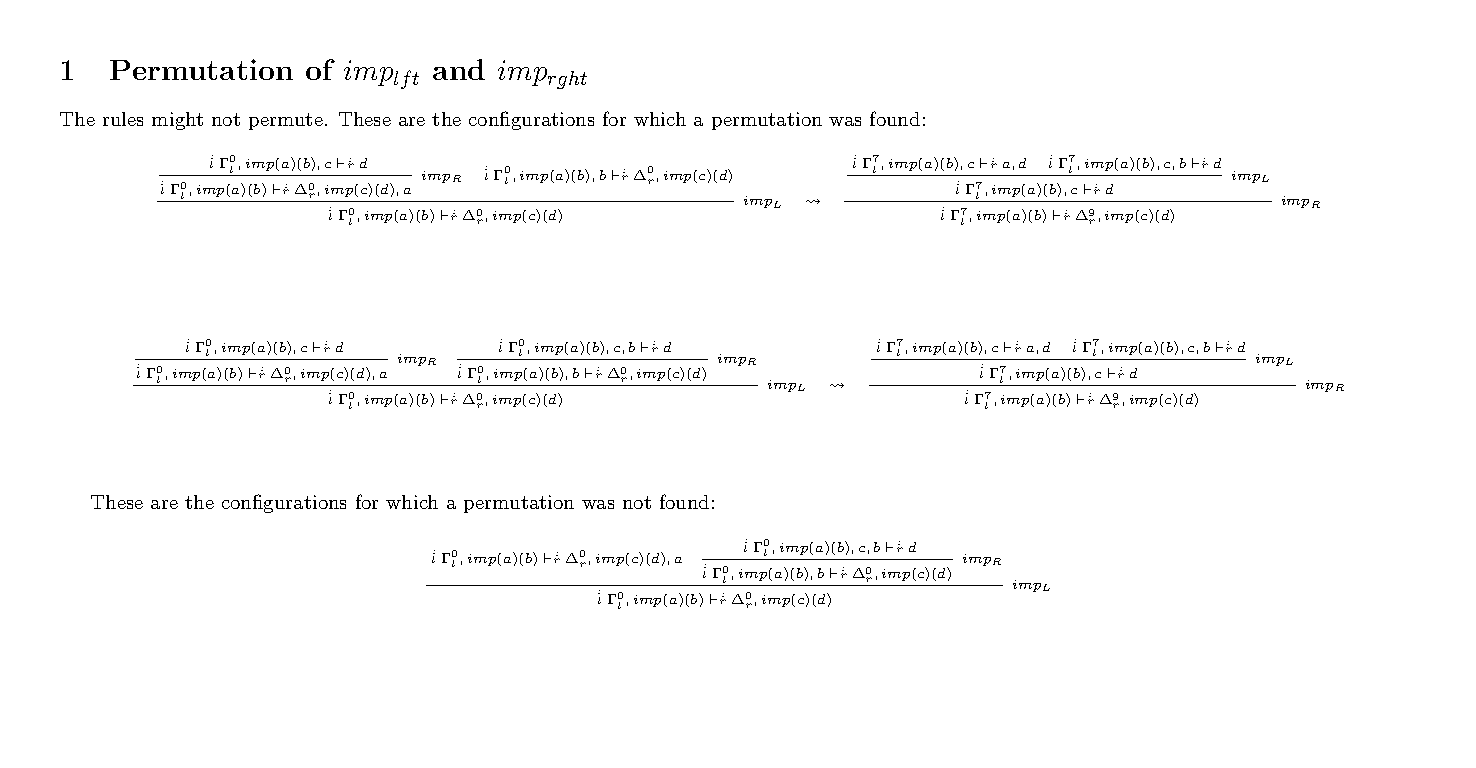
\includegraphics[scale=0.6]{imp_l_imp_r.pdf}
%\caption{Output file for the permutation of $\rightarrow_l$ over $\rightarrow_r$
%of the system MLJ.}
%\label{fig:perm_output}
%\end{figure}

\end{document}

%%%%%%%%%%%%%%%%%%%%%%% OLD STUFF, COMMENTED OUT %%%%%%%%%%%%%%%%%%%%%%%%%

% While this illustrates only one case, proving the focusing discipline, for
% instance, requires that the permutation of every pair of rules is checked. For a
% system with $n$ rules, this amounts to $2^n$ cases.
% 
% The checking of all cases is a tedious and error prone task. Moreover, the
% fact that the cases are rarely documented makes it hard for others to check the
% correctness of the transformations. The cut-elimination result for
% bi-intuitionistic logic, for example, given by Rauszer \cite{rauszer74studia}
% was later found to be incorrect \cite{crolard01tcs} exactly because one of the
% permutation lemmas was not true. An automated tool to check for these lemmas
% would be therefore of great help.
% 
% In this paper we describe such a tool. Section \ref{sec:checking} explains
% briefly the theoretical background that was implemented. Section \ref{sec:quati}
% describes the actual implementation and explains, with an example, how to use
% it. Section \ref{sec:conclusion} summarizes the results obtained and point the
% directions of future work.

% \section{Checking proof transformations}
% \label{sec:checking}
% 
% % Explain briefly the method and cite other papers.
% % This section should be small or even merged to the introduction.
% 
% Given a sequent calculus proof system, it was shown in \cite{ENTCS?} that it
% is possible to encode it, under certain conditions, in linear logic with
% subexponentials. This is a refinement of linear logic that allows an
% arbitrary (finite) number of different types of the modalities $!$ and $?$. Each
% one corresponds to a different context in the sequent of the object logic. In
% this encoding, each inference rule of the object logic corresponds to a
% formula in subexponential linear logic. This formula is called a \emph{bipole} because of its
% particular nesting of operators, and its derivation, also called a bipole, is composed by exactly one
% negative and one positive phase in the \emph{focusing} discipline. The details
% of the encoding and the format of these derivations is out of the scope of this
% paper and we refer the curious reader to \cite{llinda} and \cite{JLC paper} for
% a deeper explanation. For the moment, it is enough to know that this encoding
% has the highest level of adequacy \cite{adequacy??}, meaning that one inference
% rule in the object logic corresponds exactly to one bipole derivation in
% focused linear logic with subexponentials (SELLF).
% 
% This correspondence allows the use of SELLF as a framework to reason
% uniformly over a range of different proof systems for different logics. In
% \cite{JLC?}, the authors show how to prove the admissibility of cut and atomic
% initial rules\footnote{This method was implemented and released as the tool
% TATU (\url{https://www.logic.at/staff/giselle/tatu/}).}, and in \cite{iclp
% paper} it is shown how to use SELLF and answer-set programming to verify proof
% transformations. Quati implements the ideas on the latter work to check
% automatically whether two inference rules permute. 
% 
% \begin{definition}
% Let $\alpha$ and $\beta$ be two inference rules in a sequent calculus proof
% system. We say that $\alpha$ permutes over $\beta$ if \emph{every} possible
% derivation that has an application of $\beta$ immediately followed by and
% application of $\alpha$ (i.e. $\beta$ is above $\alpha$) can be transformed into
% a derivation where $\alpha$ is followed by $\beta$.
% \end{definition}
% 
% Using the SELLF specification of a rule, generic contexts and answer-set
% programming, we can determine all the instances of an inference rule
% application to a sequent \cite{iclp}. It is worth noting that this reasoning is
% actually done on the linear logic level. So the derivation with generic contexts
% is done in SELLF, and the models of the answer-set program specify bipole
% derivations. But because of the specifications' high level of adequacy, we can
% directly translate the bipole derivations to rules of the specified logic. A
% rewriting system is presented in \cite{iclp} for this translation.
% 
% Given this algorithm, it is possible to specify all instances of $\alpha$ on a
% generic sequent containing main formulas for $\alpha$ and $\beta$. For each of
% these instances, we can also specify how $\beta$ can be applied on its premises.
% Taking all possible combinations, we have the set $\mathcal{S}_1$ of
% derivations in which $\beta$ is immediately above $\alpha$. Repeating the
% procedure with the rules switched, we have the set $\mathcal{S}_2$ of
% derivations in which $\alpha$ is immediately above $\beta$. To check the
% permutation of $\alpha$ over $\beta$, one needs to check if a proof of each
% derivation $d \in \mathcal{S}_1$ implies in a proof of some derivation $d' \in
% \mathcal{S}_2$. The provability implication of derivations can also be
% determined via an answer-set program described in \cite{iclp}.

\begin{comment}
\section{Quati}
\label{sec:quati}

%% TODO: make a release with only the functionalities for quati to work. Put it
%% in the downloads section of google code so that we can refer to the link here.
%% Remember to put only the examples that are currently working!!
%% Write a readme file!!

Quati is implemented in OCaml\footnote{\url{http://ocaml.org/}} and makes use of
DLV\footnote{\url{http://www.dlvsystem.com/dlv/}} externally to compute minimal models for the
answer-set programs generated. It is part of a bigger project, called
\texttt{sellf}\footnote{\url{https://code.google.com/p/sellf/}} which started as an effort to
implement the focused proof system for linear logic with subexponentials
\cite{vivek's thesis}. The basic data structure is linear logic formulas,
defined in the \texttt{Term} module. Figure \ref{fig:modules} is an overview
of the modules in \texttt{sellf} used by Quati to check for permutations.

\begin{figure}
TODO: module's figure
\end{figure}

\textbf{TODO:} wait for the picture to explain in more detail the modules and how they
interact.

Quati takes as input the SELLF specification of a sequent calculus proof system.
This is done via two files, one with extension \texttt{.pl} and the other with
\texttt{.sig}. The former contains the actual specification of the proof system,
namely, the formulas corresponding to each inference rule, the subexponentials
used and their properties. The latter contains a signature declaration of the
connectives of the object logic. For example, if the logic being specified has a
connective $\wedge$, one needs to declare a predicate, say \texttt{and}, of type
\texttt{form -> form -> form}. Figure \ref{fig:input} shows an example of these
input files and Tables \ref{tbl:syntax_ll} and \ref{tbl:syntax} show the syntax of the
linear logic connectives and some keywords used in specifications.

\begin{figure}
\caption{Specification and signature files of the multi-conclusion
calculus for intuitionistic logic \textbf{mLJ}.}
\label{fig:input}
\end{figure}
%
\begin{table}
\centering
\begin{tabular}{|c|l|}
\hline
Syntax & Meaning \\
\hline
\hline
%% TODO: maybe these deserve a better explanation...
\texttt{rght A} & $\lceil A \rceil$ (represents a formula $A$ on the right side of the sequent in the object logic)\\
\hline
\texttt{lft A} & $\lfloor A \rfloor$ (represents a formula $A$ on the left side of the sequent in the object logic)\\
\hline
\texttt{form} & Type for object logic formulas.\\
\hline
\texttt{term} & Type for object logic terms.\\
\hline
\texttt{subexp} & Keyword to declare contexts.\\
\hline
\texttt{unb} or \texttt{lin} & Specifies whether a context allows contraction and weakening of its formulas.\\
\hline
\texttt{subexpctx} & Keyword to declare contexts' properties.\\
\hline
\texttt{many} or \texttt{single} & Specifies the number of formulas a context can hold.\\
\hline
\texttt{lft} or \texttt{rght} & Specifies whether a context occurs on the left or on the right side of the sequent.\\
\hline
\end{tabular}
\vspace{0.2cm}
\caption{Syntax reference for specification of systems.}
\label{tbl:syntax}
\end{table}
%
%% put the grammar of the syntax instead???
There are already a few proof systems specified in Quati, such as \textbf{LK},
LJ, \textbf{mLJ}, \textbf{LL}, etc. They were used for testing purposed
and are available for the user as examples. Quati can be downloaded at
\url{[TODO: link of the release]} as a zip containing its source code, the
examples and installation instructions. Alternatively, it can be tested using a
limited web interface at \url{https://www.logic.at/staff/giselle/quati/}.

%% Maybe show the example first???
\subsection{An example session}

We will illustrate the features of Quati using a sample run on the command line
interface. This is preferred over the web interface because it provides extra
functionality.

%% TODO: demo session on the command line
% load file
% type bipoles to print the rules
% show the latex code that's printed for one rule as the object logic rule and
% the linear logic bipole
% type permute to check permutation of two rules
%   one example that permute
%   - show the permutations as object logic rules
%   one example that does not permute
%   - show the successful and failed cases as ol rules

\section{Conclusion}
\label{sec:conclusion}

- mention the systems implemented and interesting cases of permutation

- cite the work with ramyaa about automating the specifications

- cite the automatic discovery of focusing systems

\end{comment}
